\chapter{
استفاده از شیفت‌رجیستر آماده
}
\section{
تراشه ۷۴۹۵
}
با مطالعه‌ی دیتاشیت تراشه‌ی ۷۴۹۵
یا صرفا با دانش کلی در رابطه با کارکرد قطعه و سعی و خطا می‌توان کارکرد پایه‌های این قطعه را فهمید و شیفت‌رجیستر مورد نظر را تنها با استفاده از این قطعه‌ی آماده ساخت.

در شکل
\eqref{fig:circuit5}
مداری مشابه قسمت قبلی را با استفاده از این قطعه ساختیم.

\paragraph{نکته:}
قطعه‌ی ۷۴۹۵ دارای دو کلاک مجزا برای حالت‌های بارگذاری مختلف است.
از آنجایی که فعلا ما نیازی به کلاک‌های مختلف نداریم نیازی به استفاده از این قابلیت نیست و می‌توانیم صرفا یک کلاک را به جفت ورودی‌های بدهیم.
اما مداری با کلاک‌های مختلف نیز در شکل
\eqref{fig:circuit7}
آمده است.

\begin{figure}[h!]
    \centering
    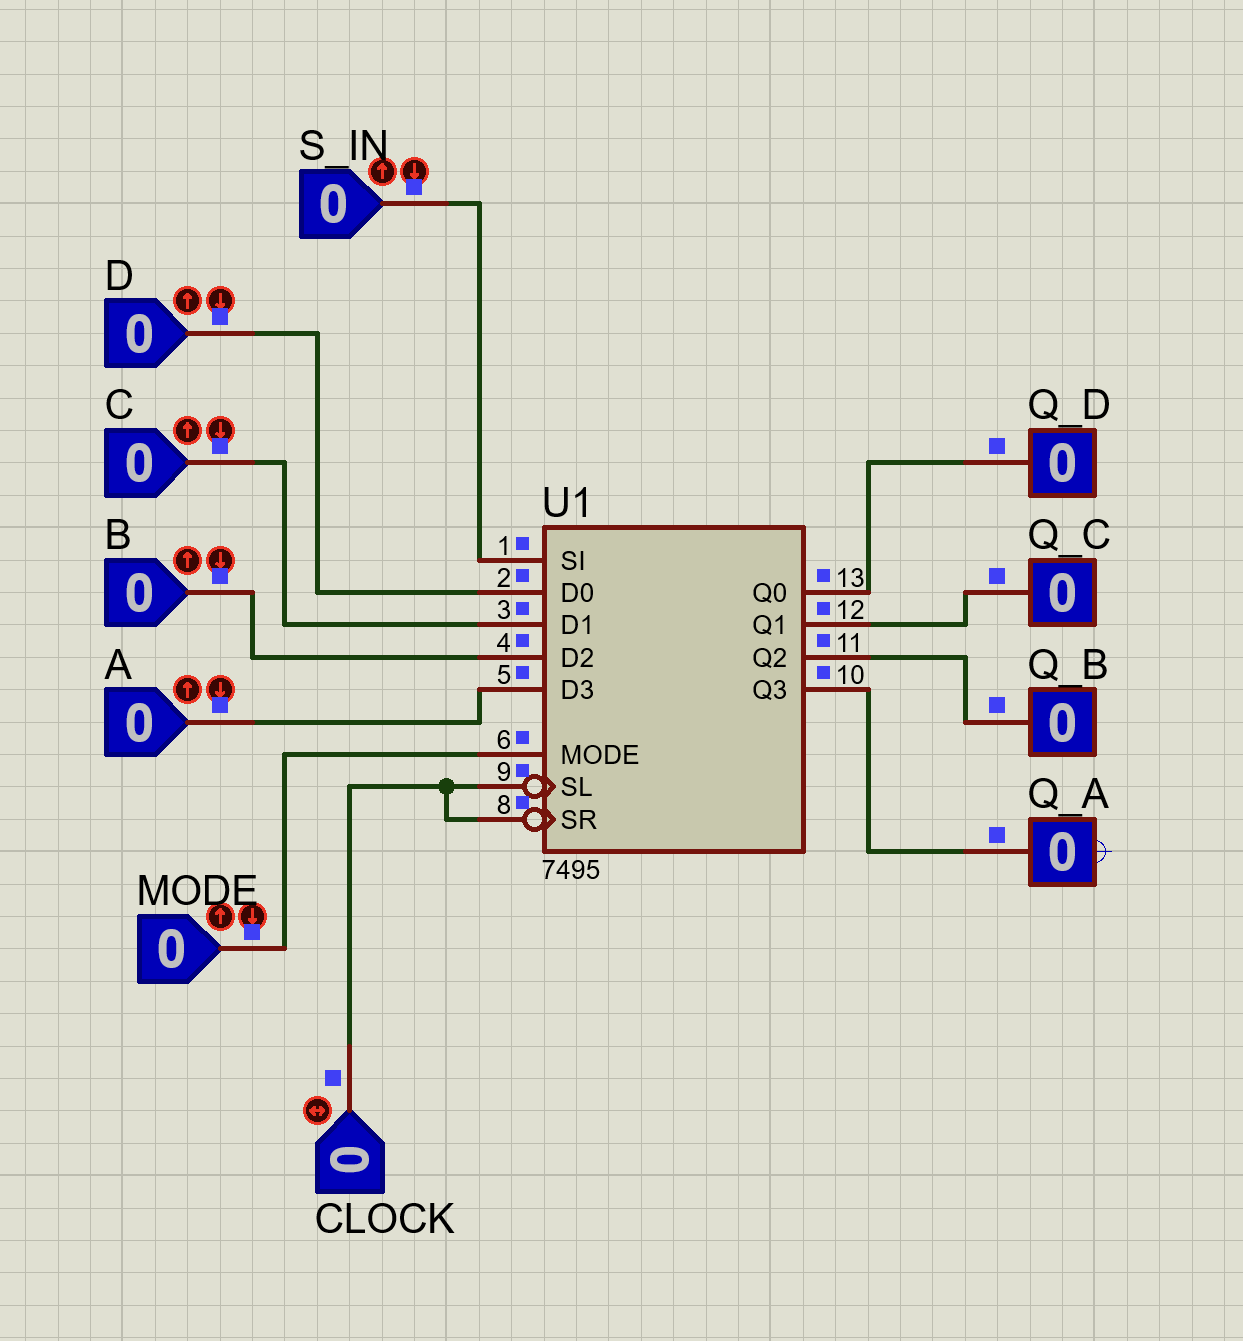
\includegraphics[width=0.6\textwidth]{part2/5.png}
    \caption{
    نحوه‌ی ساخت مدار قسمت قبل با استفاده از قطعه‌ی ۷۴۹۵
    }
    \label{fig:circuit5}
\end{figure}


\begin{figure}[h!]
    \centering
    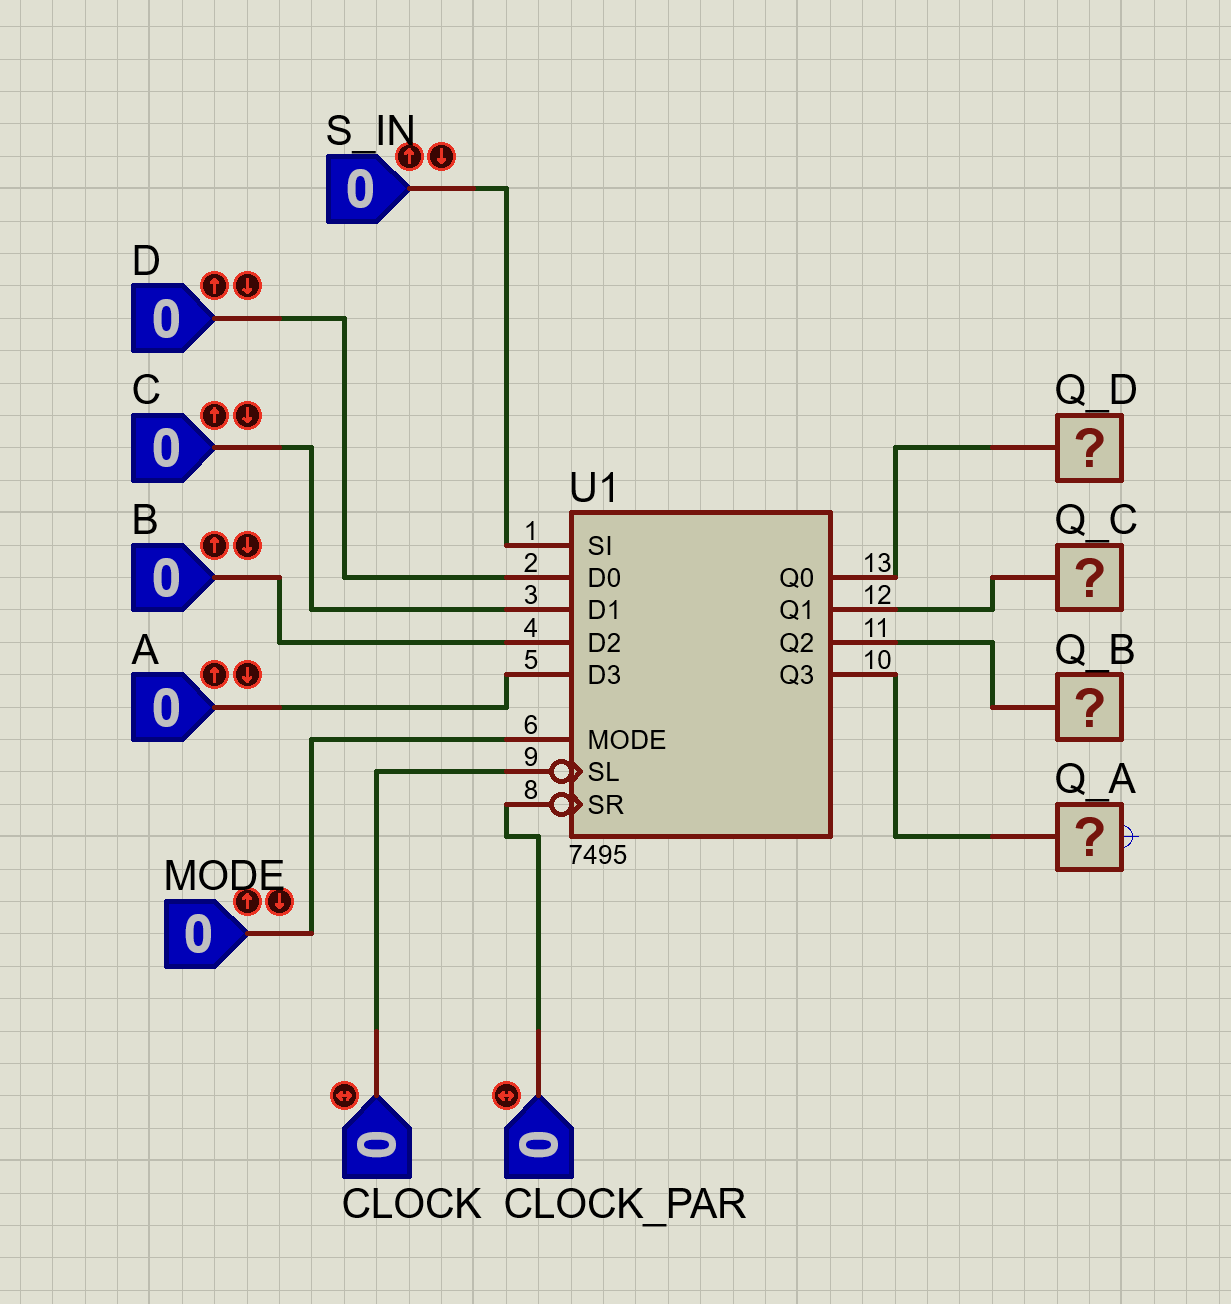
\includegraphics[width=0.6\textwidth]{part2/8.png}
    \caption{
    مدار با کلاک‌های متفاوت
    }
    \label{fig:circuit7}
\end{figure}

کارکرد هر پایه و خروجی با لیبلی روی آن مشخص شده است.


\section{
مدار شناسایی رشته
}
همانطور که در درس مدارمنطقی آموختیم، ساخت مدار تشخیص یک زیررشته‌ی 
خاص در یک رشته با شیفت‌رجیستر کار بسیار ساده‌ای است.
کافی است یک شیفت‌رجیستر به طول قطعه‌ای که می‌خواهیم تشخیص دهیم داشته باشیم و رشته‌ی اصلی را از آن عبور دهیم.
هر وقت که زیررشته در رشته‌ی اصلی وجود داشتِ، لحظه‌ای وجود دارد که بیت‌های شیفت‌رجیستر برابر با رشته‌ی مورد نظر هستند و بنابراین با تعدادی گیت‌اند و نات
(یا قطعه‌ی مشابه مثلا دیکودر)
می‌توانیم وجود آن را تشخیص دهیم.

در اینجا چون وجود هر کدام از زیررشته‌ها کافی است، باید نتایج
گیت‌های
AND
را با هم
OR
کنیم.
ممکن است با رسم جدول کارنو بتوان ساده‌سازی‌هایی بر مدار نهایی انجام داد، اما این کار به شدت از خوانایی مدار می‌کاهد و ضمنا کار دشواری است.
دلیل دیگر هم این که در پروتئوس و محیط‌های آزمایشگاهی می‌توانیم از گیت‌هایی با چند ورودی استفاده کنیم که تئوری‌های معمول و جدول کارنو این موضوع را در نظر نمی‌گیرند.

نتیجه‌ی این آزمایش در تصویر
\eqref{fig:circuit6}
آمده است.


\begin{figure}[h!]
    \centering
    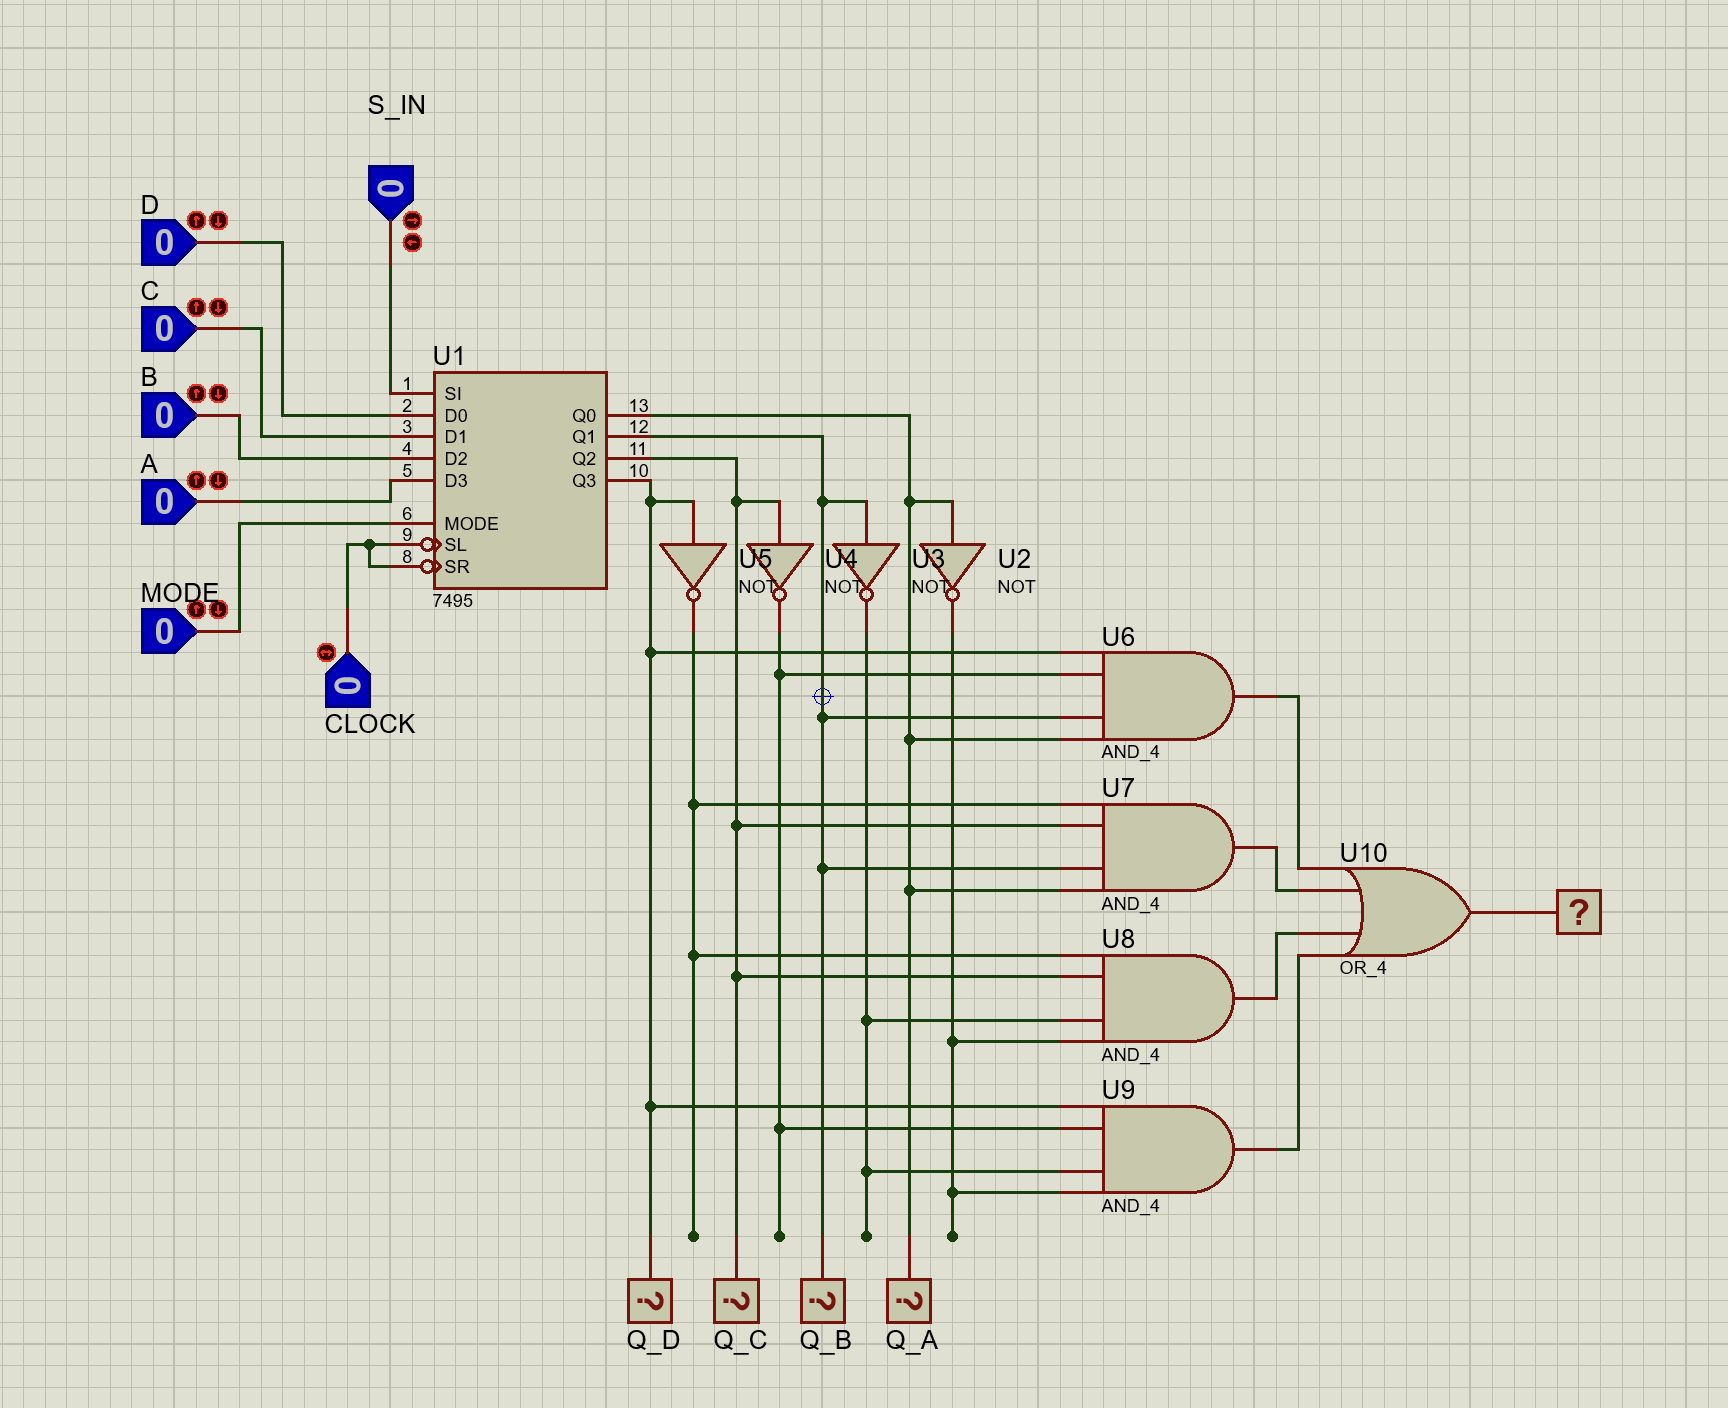
\includegraphics[width=\textwidth]{part2/9.png}
    \caption{
    مدار تشخیص زیررشته
    }
    \label{fig:circuit6}
\end{figure}
